\scanpage{119}
dans ce cas la flèche horizontale sera bien un isomorphisme \deleted{\unsure{dans|donc}} après application de $\tau_\omega$\ldots\ En effet, \unsure{ch.que|chaque} $C_*^{i*}$ est une résolution de $(S_k^i)_*$ (dans $(\mathrm{Ss})$), jusqu'au degré $p$ si $i$ est assez grand p.r. à $p$, \unsure{donc}\ldots.

\deleted{On} Regardons la condition d'isomorphie (après application de $\tau$) pour la flèche verticale, elle \deleted{est satisfaite} est conséquence de la condition suivante (et sans doute équivalente)

% slanted
\margin{On peut \deleted{\unsure{peut-être}} affaiblir (4), en prenant ``flasque jusqu'en une \unsure{dimension|générateurs} donnée'' (du côté $\mathrm{Ss}$)}
(4) Pour tt $i\geq0$ considérer les \inserted{groupes $1/2$ simpl.} $C_*^{ip}$ $(p\geq0)$ et soit $\pi(i)$ le plus petit entier (s'il existe) tel que $C_*^{ip}$ ne soit pas flasque ($\pi(i)=+\infty$ sinon), \deleted{\unsure{ceci veut}} i.e. que son \uline{\unsure{hologie|homologie|faisceaux}} $1/2$ simpliciale \inserted{(pour $\partial$)} soit non nulle. On veut que $\pi(i)\longrightarrow+\infty$ quand $i\longrightarrow+\infty$.

\figure{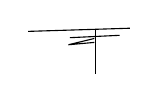
\begin{tikzpicture}[x=1cm,y=1cm]
 \draw (-.65,.18)--(.64,.22); \draw (.2,.20)--(.2,-.36);
 \draw (-.12,.1)--(.51,.13); \draw (.19,.09)--(-.14,.01)--(.19,.04);
\end{tikzpicture}}

On aimerait prouver un th. d'unicité (\unsure{ou.|ou} déjà l'existence\ldots)

Les $C_*^{**}$ ayant les structures précisées (au besoin en oubliant d'abord la structure p.d.) et satisfaisant
% archive sheet number: 118
